\chapter{Biophysical background}
Proteins are one of the essential components of living systems. Along with nucleic acids, polysaccharides, and lipids, proteins constitute the macromolecules that have important roles in biology. 
Nucleic acids, in the form of DNA and RNA, store and distribute the genetic information as needed. Of particular importance is the information that determines the sequences of amino acids that characterize the proteins. Proteins contribute to the structure of an organism and execute most of the tasks required for it to function. Proteins even form part of the complex mechanism by which they are synthesized. Polysaccharides, linear and branched-chain polymers of sugars, provide structural elements, store energy, and when combined with peptides or proteins, play an important role in antigenicity and, more generally, in cellular recognition. Lipids, which include molecules such as fatty acids, phospho- lipids, and cholesterol, serve as energy sources and are the most important components of the membrane structures that organize and compartmentalize cellular function.

\section{Basics of protein structure and their functionality}
\subsection{Macromolecules}
Molecules are generated by the formation of covalent bonds between pairs of atoms, in which the two atoms share electrons. A covalent bond forms when atoms individually do not have enough electrons for a complete octet: if two atoms can complete their octets by sharing electrons, they can do so by forming a covalent bond. Covalent bonds can be explained only by quantum mechanics, but here it is necessary simply to recognize that covalent bonds are generally not broken in isolation under most conditions experienced in molecular biology. When a covalent bond is broken, as in a chemical or enzymatic reaction, it is generally exchanged with another covalent bond to a different atom. Consequently, covalent bonds define the structures and properties of small molecules, and those of large molecules are determined by the covalent structures of the smaller substituents from which they are made.

The most important molecules in biology are proteins and the nucleic acids deoxyribonucleic acid (DNA) and ribonucleic acid (RNA); all are macromolecules characterized by their very large sizes and high molecular weights. These giant molecules can contain many thousands, millions, even billions, of atoms. Fortunately, these macromolecules are polymers, produced by linking together in a linear fashion only a few relatively simple monomers: four nucleotides in the case of DNA and RNA, and 20 amino acids in the case of proteins. In each of these cases, each residue, $i$, of the chain consists of two parts: group $X$ comprises the backbone and is the constant, repeating part of the polymer, while the side-chains (A, B, C, ...) attached to the backbone are variable:

\begin{figure}[h]
\centering
\begin{minipage}[t]{0.8\textwidth}
\centering
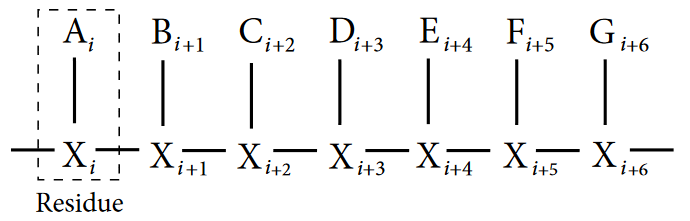
\includegraphics[width=0.7\textwidth]{Polymer.PNG}


\label{fig:Polymer}
\end{minipage} 
\end{figure}

The side-chains connected to the backbone are all the same in homopolymers, as in carbohydrates or polymers made chemically, but they are variable in copolymers; the natural proteins and nucleic acids are extreme examples with several different types. Normally the individual residues are indexed from 1 to $n$, starting from one end of the polymer chain and finishing at the other. The bonds between the residues are numbered similarly, with bond $i$ joining residues $i$ and $i + 1$; there are then $n – 1$ bonds linking the $n$ residues. Normally the backbone primarily has a structural role, while the side-chains contain the functional groups. In spite of the enormous sizes of proteins and nucleic acids, it is possible to determine their detailed covalent structures because, knowing the detailed structures of all the possible monomers, it is necessary only to determine their linear sequence in the polymer.
The detailed structures of the monomers are extremely important, because they determine the global properties of the macromolecule. They occur many times in the polymer, and their structures are multiplied many times over. Many of the monomers occur in only one of several possible isomers; for example natural proteins are composed solely of $l$-amino acids and nucleic acids of $d$-ribose or $d$-deoxyribose. While these details of the structure might seem very minor and mundane, they have extremely important consequences for the three-dimensional (3-D) structures of biopolymers and their functions. These consequences even extend to the macroscopic level; for example, the left/right asymmetry of all but the simplest microorganisms is believed to result from asymmetry at the atomic level of certain molecules.

1.4. STRUCTURE DATABASES: STRUCTURES ON THE WEB
Structure databases contain the 3-D structures of biological macromolecules determined by X-ray
crystallography and NMR. The primary structure database is the Protein Data Bank (PDB), an
archive of all publicly available 3-D structures of proteins, nucleic acids, carbohydrates, viruses and
biomolecular complexes. The PDB is basically a collection of text files, each containing a structure
entry deposited by those who determined the structure. An entry file consists of (1) text information
of definition, source, references and comments, (2) the sequence information, (3) the secondary
structure information and (4) the 3-D coordinates of all the atoms, as well as crystallographic structure
factors and NMR experimental data. There is an efficient search engine for finding files of the desired
structures. Other useful structure databases include the Nucleic acid Database (NDB) for nucleic
acids and the Cambridge Structural Database (CSD) for organic and metal–organic compounds. The
World Wide Web addresses for these databases are given in Table 1-1. The majority of databases in
molecular biology are publicly available and freely accessible via the Web.

\subsection{Protein structure}
POLYPEPTIDE STRUCTURE
Polypeptide chains make up proteins, which are one of the most important classes of biological
macromolecules, having both structural and catalytic roles. Polypeptide chains are built up during
their biosynthesis from basic building blocks of 21 different amino acids. The amino acids are linked
together in a linear polypeptide chain by forming peptide bonds between them, in an order ordained
by the nucleotide sequence of the corresponding gene for the protein (Section 7.5.F). These 21 amino
acid residues can also be modified post-translationally in very many different ways, to produce even
more variety. The amino acid sequence, appropriately known as the primary structure, identifies a
protein unambiguously, determines all its chemical and biological properties, and specifies (indirectly)
the higher levels of protein structure (Chapters 8 and 9).

7.1. POLYPEPTIDE CHAINS\footnote{A word on nomenclature: a peptide is a shortpolymer of a few amino acid residues with a defined sequence; it usually has properties that are close to those expected from just its constituent amino acids. A polypeptide is a longer chain, with more amino acid residues and a defined sequence; it is usually assumed to remain unfolded and to have no special chemical or physical properties. A polyamino acid has sequences of varying lengths produced by nonspecific random polymerization of one or a few amino acids. A protein is a polypeptide chain with a defined length and amino acid sequence that adopts a specific folded conformation and has special physical and chemical properties.}
Twenty of the amino acids used to synthesize natural proteins have the general structure:

\begin{figure}[h]
\centering
\begin{minipage}[t]{0.325\textwidth}
\centering
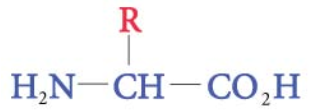
\includegraphics[width=\textwidth]{GenericAminoAcids.PNG}


\label{fig:GenericAminoAcids}
\end{minipage} 
\end{figure}

they differ only in the chemical structures of the side-chain, R. The amino group and the carboxyl
group give this class of compounds its name. At physiological pH values, both groups are ionized,
and this zwitterion is the common form of the amino acid in solution. The exceptional amino acid,
proline, differs in that its side-chain is bonded to the N atom of the amino group, which is then a
secondary amine, and proline is an imino acid:
The central C" atom is asymmetric in 20 of the amino acids and is always the L-isomer:
The L-isomer can be readily identified by looking down from the H atom to the C atom and
remembering the "CORN rule": the other groups should occur in the clockwise sequence CO, R
(side-chain) and N. Glycine is the exception, in that its side-chain is simply another H atom, so the
C" atom is not chiral.
Amino acids are linked together by peptide bonds formed by condensation of the a-carboxyl group
of one amino acid with the a-amino group of another, producing a dipeptide (Figure \ref{fig:PeptideFormation}). Repeated
condensation of additional amino acids produces tripeptides, tetrapeptides, and so on.

\begin{figure}[h]
\centering
\begin{minipage}[t]{0.8\textwidth}
\centering
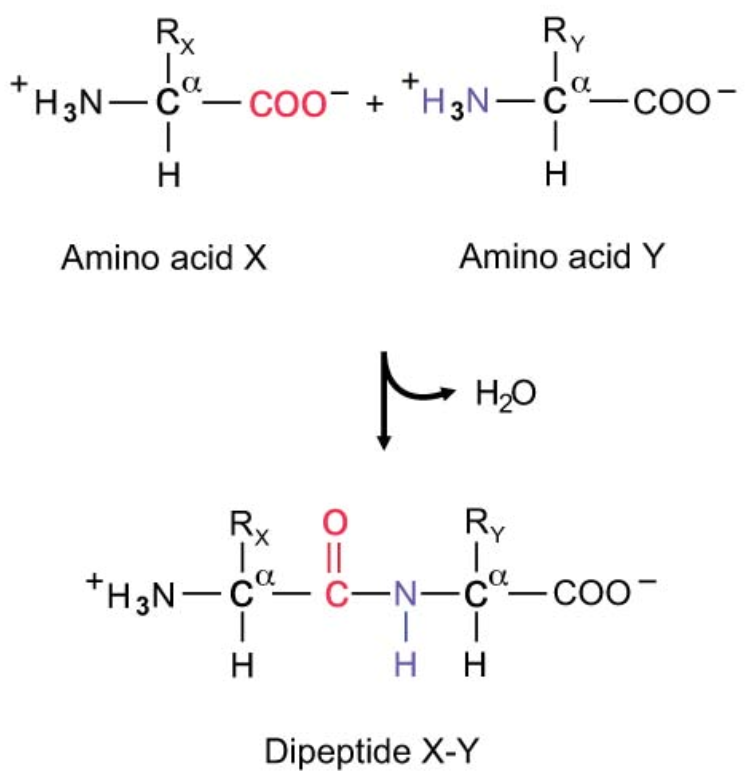
\includegraphics[width=0.6\textwidth]{PeptideFormation.PNG}

\caption{\small{General scheme for formation of a dipeptide XY from two amino acids, X and Y, by reaction of the carboxyl group of amino acid X with the amino group of amino acid Y. The R group attached to Ca is variable depending on the type of amino acid: R, and R, \cite{chong2015dissecting}.}}

\label{fig:PeptideFormation}
\end{minipage} 
\end{figure}


POLYPEPTIDE CONFORMATION
The structures of all molecules extend to three dimensions. Two-dimensional (2-D) chemical
representations usually suffice for small molecules because their three-dimensional (3-D) structures
are defined reasonably well by the fixed bond lengths and bond angles of their covalent structures.
These representations are not sufficient for larger molecules, however, because rotations about
the many covalent bonds dramatically alter the relative positions of all the atoms. 3-D aspects of
structure are especially important for polymers such as nucleic acids and proteins, in which many
bonds can rotate. Polymers have an intrinsic tendency to be very flexible, when no one structure,
or conformation (Section 1.2), is sufficiently more stable than all the others to predominate, but
nevertheless many biological macromolecules, especially the proteins and nucleic acids (Chapters 2,
4 and 9), tend to adopt single, stable conformations.
The abilities of polypeptide chains to adopt a wide variety of 3-D conformations is crucial so that they
can carry out their many different functions (Chapters 12–15). These conformational properties of
polypeptide chains are controlled to a great extent by the flexibility of the polypeptide backbone and
by local interactions with amino acid side-chains, which are described in this chapter.

8.2. RANDOM-COIL POLYPEPTIDE CHAINS
The substantial flexibility of the polypeptide chain gives it significant conformational entropy (Section
1.3) and makes the random coil the most favored conformation under many conditions. Most studies
of random polypeptide chains have been done with polyamino acids, in which one type of amino acid
is polymerized into a homopolypeptide chain. Yet it is not clear that any polypeptide chain adopts
a completely random-coil conformation, as various interactions can usually be observed, especially
between chemical groups close in the covalent structure. Many unfolded proteins that previously were
thought to approximate random coils are now thought to contain significant amounts of nonrandom
conformation, like that observed in poly(Pro) II (Section 8.3.D), but this might just be the most
favorable stereochemistry for the polypeptide chain.

PROTEIN STRUCTURE
Most dynamic activities in cells and organisms are caused by proteins, and the key to understanding
these phenomena is their structures. Protein structures, however, consist of many atoms, often
thousands, and can be extremely complex. Natural proteins are also folded into precise threedimensional
(3-D) structures and are very different from random-coil forms of the polypeptide chain
(Section 8.2), in that most of their covalent bonds adopt a single dihedral angle (Section 1.2.B) and
Cys residues pair in specific disulfide bonds (Section 7.2.1.5), rather than the spectrum possible with
disordered polypeptide chains (Table 7-3); this generally results in a folded conformation that can be
considered unique. It is also very compact. No changes in covalent structure need occur when these
folded conformations are adopted, except for the disulfide bonds that might be formed between Cys
residues (Section 7.2.1.5); therefore the folded structure represents just one conformation of the many
that are possible with a disordered polypeptide chain. With 20 different amino acid residues having
diverse physical and chemical properties, a huge variety of protein sequences and conformations are
possible. Some proteins are globular and water-soluble, others exist buried within membranes, while
others adopt elongated and extended structures that serve primarily structural roles (Section 8.5).
Protein structure is most impressive in its diversity.
Each protein is identified uniquely by its amino acid sequence, which is determined by the
sequence of the gene from which the protein is produced, using the genetic code (Section 7.5.F). The
amino acid sequence determines all further aspects of the structure of the protein and, consequently,
its functions. It has become customary to dissect protein structure into four levels (Figure 9-1).
The primary structure is the amino acid sequence. The secondary structure is any regular local
structure of a linear segment of polypeptide chain, such as a helix or an extended strand (Section
8.3). The tertiary structure is the overall topology of the folded polypeptide chain. The quaternary
structure is the aggregation of the individual polypeptides by specific interactions between them.
As more protein structures have been determined, two intermediate levels of structure have become
apparent; one comprises several elements of secondary structure packed together and is known as the
supersecondary structure or motif; the other is the domain, which can be one self-contained part
of a tertiary structure.
Details of virtually all the known structures of proteins can be obtained from the Protein Data Bank
(PDB; www.rcsb.org). They can be viewed most readily online using the program Jmol at http://
firstglance.jmol.org.

\begin{figure}[h]
\centering
\begin{minipage}[t]{0.875\textwidth}
\centering
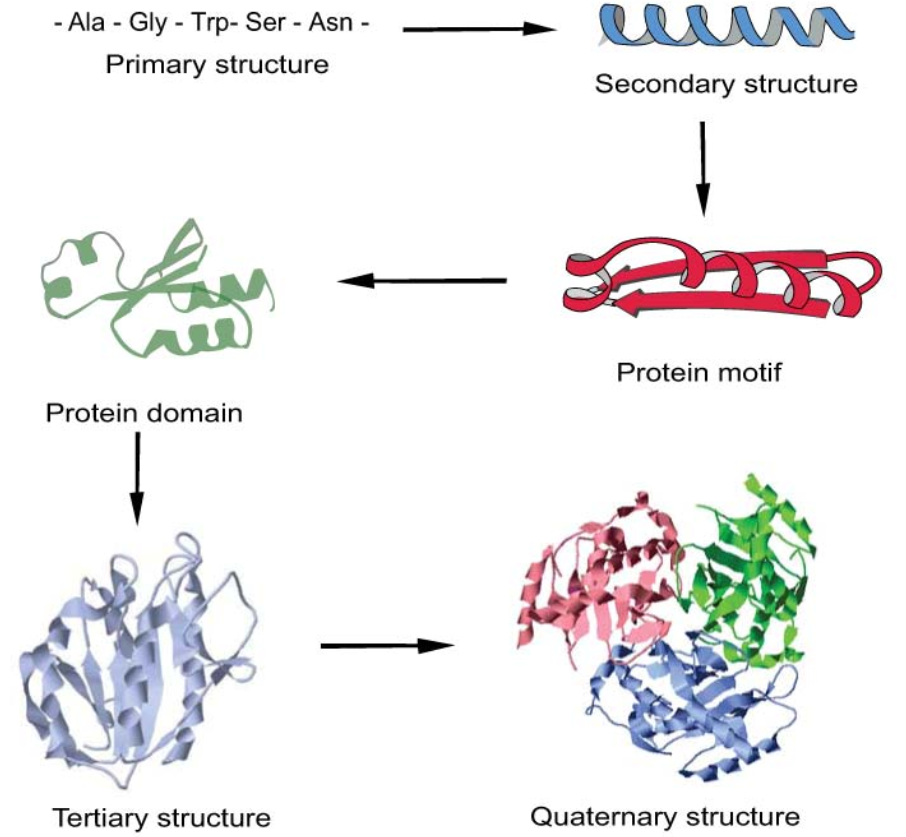
\includegraphics[width=0.9\textwidth]{ProteinStructure.PNG}

\caption{\small{Different levels of  protein structure, from primary to quaternary. Helices are depicted as coils and P-strands as arrows. The primary structure is the amino acid sequence of the polypeptide chain. The secondary structure example shown is an a-helix; the protein motif is  a pap motif, where P is a P-strand, a an a-helix and the motif produces a parallel P-sheet. The protein domain is a folded structure that is stable in isolation. The tertiary structure is the folded structure of a complete polypeptide chain, in this case that of flavodoxin. The quaternary structure is produced by the aggregation of multiple polypeptide chains; in this case it is the homotrimer of  chloramphenicol acetyltransferase. 
\cite{chong2015dissecting}.}}

\label{fig:ubq}
\end{minipage} 
\end{figure}

\begin{figure}[h]
\centering
\begin{minipage}[t]{0.6\textwidth}
\centering
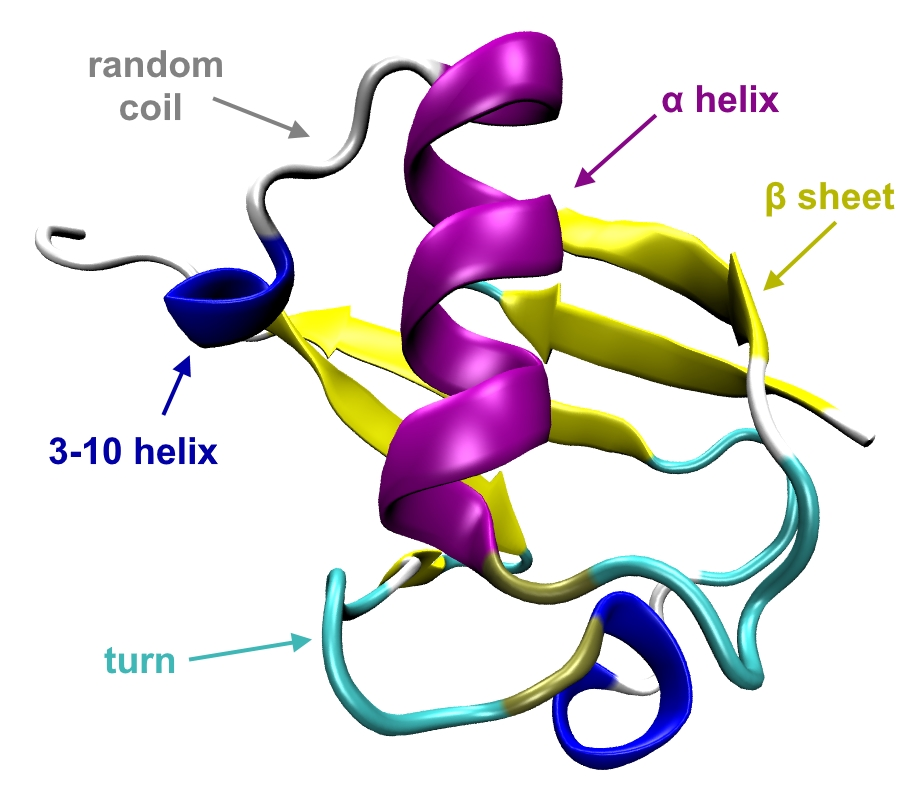
\includegraphics[width=\textwidth]{ubq-label.jpg}

\caption{\small{}}

\label{fig:ProteinStructure}
\end{minipage} 
\end{figure}


\section{Basics of protein structure and their functionality}



\section{Protein-ligand binding}
%\section{Ligand binding process}
The biological functions of macromolecules almost invariably depend upon their direct physical
interaction with other molecules. All organisms and cells survive only because they interact
effectively with their environments. Extraneous molecules must be distinguished as either useful or
dangerous and dealt with accordingly. Organisms have sophisticated sensory organs for being aware
of their environments. At a lower level, all cells have a variety of receptors for different molecules
for this purpose. Virtually every small molecule in a cell was first bound specifically by the enzyme
that produced it or by the receptor on the cell that enabled it to enter that cell. Every aspect of the
structure, growth and replication of an organism depends upon proteins binding small molecules,
other proteins, nucleic acids, polysaccharides or lipids. Of crucial importance is the specificity of such
interactions. In the crowded interior of a cell, each molecule must interact only with the appropriate
molecules and not with any of the others that are present, often in extremely high concentrations.
The following discussion will be general but will apply primarily to proteins binding smaller ligands,
such as their substrates for enzymatic reactions, although the catalytic events that take place after
binding on the enzyme will be saved for Chapter 14. The interactions between nucleic acids and
proteins are described in Chapter 13; base-pairing interactions between complementary strands of
DNA and RNA are described in Chapter 5, and their interactions with small molecules are described
in Sections 2.5 and 14.6.
Only binding to specific sites on a protein will be considered here, and phenomena such as the
electrostatic binding of counterions to a polyanion or polycation (Section 2.3) will not be considered
here as ligand binding. Likewise, little attention will be given to interactions with normal components
of the solvent, such as water molecules and co-solvents in the case of water-soluble proteins and lipids
in the case of membrane proteins. These interactions are not fundamentally different but they do
not occur at specific sites on the protein and are generally weak, occurring only because the solvent
molecules are present at high concentrations
\cite{chong2015dissecting}

12.1. GENERAL PROPERTIES OF PROTEIN-LIGAND INTERACTIONS
Proteins usually bind only very specific ligands and can discriminate between closely related
molecules. This specificity is usually crucial for their biological functions. Proteins are generally
classified according to the purpose and consequences of their binding; examples are structural
proteins, enzymes, repressors, lectins, toxins, immunoglobulins, hormones, receptors, membrane
transport proteins and proteins of motility. The physical principles of the interactions are similar in
all these cases. The following discussion focuses on the protein; whatever molecule it interacts with,
even if another protein, is designated the ligand. A protein with its ligand bound is known as the holo
form; that without the ligand is the apo form. Some examples of specific complexes are illustrated in
Figure 12- 1.

\section{The free-energy landscape and conformational entropy}
%\section{Hydration water}

The understanding of how ligands bind to proteins is of fundamental importance in biology and medicine.\footnote{The structures of protein-ligand complexes at atomic resolution make possible, for example, the design of small-molecule drugs for the treatment of disease \cite{dunn2001protein}.} Indeed, the protein-ligand interactions are crucial for the determination of the biological functions and, as a consequence, these interactions underlie almost all processes occuring in living organisms. In fact, every aspect of the structure, growth and replication of an organism depends in general on the way the proteins bind ligands (i.e. small molecules, nucleic acids, peptides, other proteins, polysaccharides or lipid) \cite{creighton2010biophysical}.

The association processes that bring to the formation of the binding between a protein and its ligand, also known as complexation, occurs when the free-energy of the whole system (protein, ligand and solvent) is lower for the complexed state, $G^\text{(c)}$, than for uncomplexed one, $G^\text{(uc)}$. Defining the difference between $G^\text{(c)}$ and $G^\text{(uc)}$ as $\Delta G$, it is possible to divide $\Delta G$ into the following two terms:
\begin{equation*}
\label{free-en}
\Delta G = G^\text{(c)} - G^\text{(uc)} = \Delta H - T \Delta S
\end{equation*}
where $\Delta H$ is the change in enthalpy due to the electrostatic interactions, while $\Delta S$ is the change in entropy due to the variation of the number of microscopic configurations for the whole system that corresponds to the new macroscopic state, namely, the solvated protein-ligand complex.
%\begin{align*}
%\label{c-uc}
%&\Delta G < 0 \quad \Longrightarrow \quad \text{\textit{the complex state is stable}} \\
%&\Delta G > 0 \quad \Longrightarrow \quad \text{\textit{the uncomplex state is stable}}
%\end{align*}

Indeed, while studying this association processes, it is useful to identify the favorable and unfavorable contributions to the change in the free-energy of the system. Most of the unfavorable contribution is due to the loss of the three translational and three rotational degrees of freedom that lead to a considerable decrease of the entropy of the system. Generally, it is assumed that this contribution is offset by favorable enthalpy of binding and entropic contributions, such as the hydrophobic effect, changes in the protonation state and solvent or counterion release. Nevertheless, there are other mechanisms, due to the creation or suppression of new internal degrees of freedom in the complex, that induce a change of the intrinsic entropy of the association by which a significant amount of entropy can be lost or recovered \cite{tidor1994contribution}. For this reason, it useful to divide $\Delta S$ in two contributions:
\begin{equation*}
\label{entropy-variation:total}
\Delta S = \Delta S_\text{intr} + \Delta S_\text{solv}
\end{equation*}
where $\Delta S_\text{solv}$ is the entropy change arising from accompanying modifications of interactions with the solvent, while $\Delta S_\text{intr}$ is the intrinsic change of the entropy involved in creating a dimer from two separate molecules \cite{steinberg1963entropy}. In particular, $\Delta S_\text{intr}$ represents the variation of the entropy due to the change of the number of configurations for the protein-ligand system upon the complexation (without considering the solvent) and, because of that, $\Delta S_\text{intr}$ is usually known as $\Delta S_\text{config} = S_\text{config}^\text{(c)} - S_\text{config}^\text{(uc)}$, where $S_\text{config}^\text{(c)}$ and $S_\text{config}^\text{(uc)}$ are the configuration entropy of the complexed and uncomplexed state, respectively. 

For each of these states, the configurational entropy represents a measure of the extent of the configuration space accessible to the internal degrees of freedom of the protein-ligand subsystem. In this way, the concept of configurational entropy is strongly connected to that of free-energy landscape and, as a consequece, a full characterization of the protein-ligand free-energy landscape is of fundamental importance to understand the relationship between the configurational entropy and the protein structure and the variation of these quantities upon ligand binding and conformational change. Unfortunately, the configurational entropy is known as one of the most difficult thermodynamic quantities to estimate and the characterization of the protein free-energy landscape is a difficult task due to its complexity and, in particular, to the fact that it is rugged, i.e., it comprises numerous local minima separated by low free-energy barriers \cite{chong2015dissecting}. 

In this regard, it was a keen insight to suppose that the protein configurational entropy $S_\text{config}$ may be characterized just by two terms, namely: 
\begin{equation*}
\label{entropy-variation:configurational}
\Delta S_\text{intr} \equiv \Delta S_\text{config} = \Delta S_\text{conf} + \Delta S_\text{vib}
\end{equation*}
where  $S_\text{conf}$ is the conformational components of the configurational entropy associated with the number of accessible free-energy wells \footnote{Sometimes, specially studying the protein folding phenomena, $\Delta S_\text{config}$ and  $\Delta S_\text{conf}$ might be used interchangeably even if they are not the same. This is why, in the protein folding process usually $\Delta S_\text{vib} \simeq 0$, hence $\Delta S_\text{conf} \simeq S_\text{conf}$ \cite{karplus1987configurational}.}, whereas $S_\text{vib}$ is the vibrational component that reflects the average width of the individual wells \cite{chong2015dissecting, karplus1987configurational}.%\footnote{Although attempts to dissect the relative magnitudes of different thermodynamic effects have been criticized as not formally correct, it remains helpful in understanding protein stability to estimate these individual contributions 
%\cite{doig1995side}.}.

\begin{figure}[h]
\centering
\begin{minipage}[t]{0.8\textwidth}
\centering
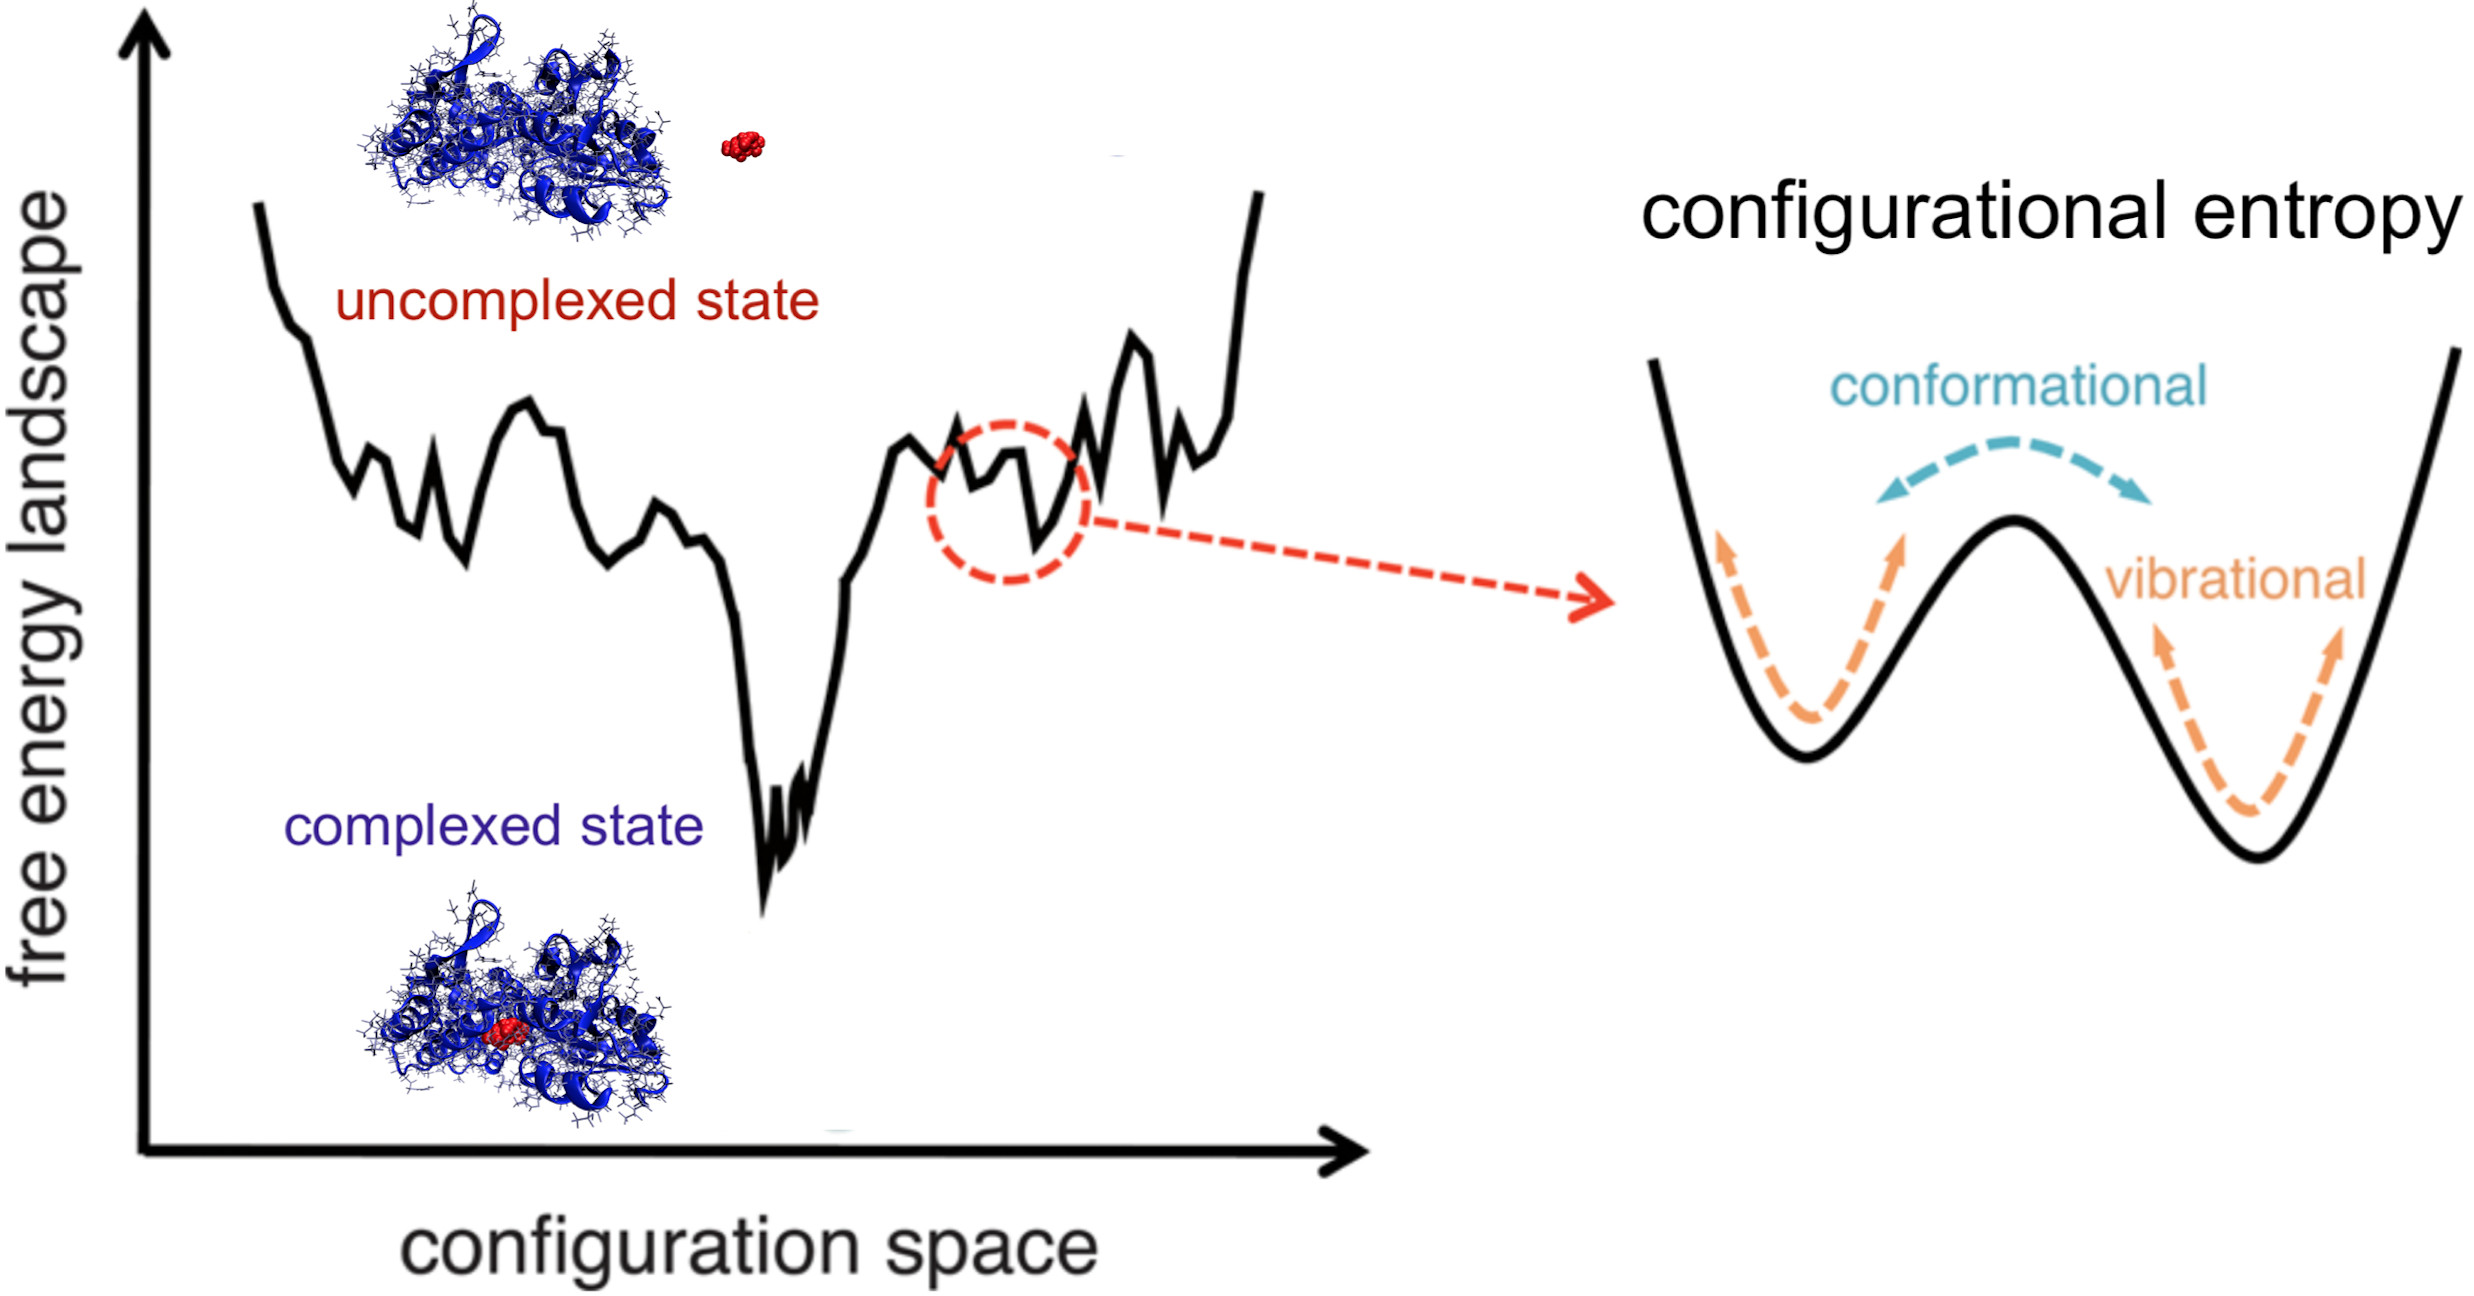
\includegraphics[width=0.93\textwidth]{free-en-landscape.jpg}

\caption{\small{Schematic representation of the free-energy landscape. Protein dynamics on the free-energy landscape can be described as a series of vibrational dynamics within individual wells and intervening conformational transitions between them \cite{chong2015dissecting}.}}

\label{fig:generation-of-microcan_state}
\end{minipage} 
\end{figure}

This subdivision of $\Delta S_\text{config}$ in two different contributions was suggested for the first time in 1981 by Karplus and Kushickt \cite{karplus1981method}. Although, in 1994, Mark and van Gunsteren criticized these types of models that attempt to decompose the free-energy into a sum of several contributions arising from different thermodynamic effects \cite{mark1994decomposition}, it has been shown that meaningful decompositions are possible and, if made carefully, they can be very useful \cite{lazaridis2002thermodynamics}.

%In 1987, Karplus et all., studying the protein denaturation, shown that, even if the $S_\text{vib}$ is typically an order of magnitude larger than $S_\text{conf}$ whether the protein is folded or not, the most important change on folding is due to $\Delta S_\text{conf}$ because the $S_\text{vib}$ is essentially the same for a protein in its native conformation and for a single conformer of the denatured polypeptide chain (i.e. $\Delta S_\text{vib} \simeq 0$ upon denaturation). 
%However, they noticed that the large magnitude of $S_\text{vib}$ raises the possibility that it may have to be considered explicitly in some cases. This is most likely when apparently small perturbations are made on the protein and a quantitative estimate of the entropy change is required. One such case is exactly the ligand binding process 
%\cite{karplus1987configurational}.

%The aim of this thesis is to evaluate of the conformational entropy change upon the complexation of a particular protein-ligand system, evaluating its conformational entropy change taking into account the effect of the formation on the binding on the hydration water.

%The aim of the thesis is to study, with molecular dynamics simulations, the association process for a specific protein and ligand system to evaluate the resulting change of conformational entropy of the system and the consequences of this change on the hydration water. Molecular Dynamics simulations are used to obtain an atomistic detail of this process. The protein and the ligand chose for the simulation are:

\vspace{0.45cm}

The objective of the thesis is to study, with molecular dynamics simulations, the protein-ligand binding in a specific case to evaluate the change of the conformational entropy upon the complexation taking into account the effect of the hydration water. Molecular Dynamics simulations are used to obtain an atomistic detail of this process.
The protein and the ligand chose for the simulation are:
\begin{center}
\begin{minipage}{0.7\textwidth}
\begin{itemize}
\item[] \textbf{Protein:} Maltose-Binding Protein (MBP)
\vspace{-0.2cm}
\item[] \textbf{Ligand:} Maltose
\end{itemize}
\end{minipage}
\end{center}
MBP and Maltose have been chosen in order to compare some of the simulations' results with the measurements of inelastic neutron scattering performed on these systems by A. Paciaroni and colleges at ILL, not yet published.\footnote{MBP is a well studied model protein that plays an important role in the metabolism of Escherichia coli, e.g., in the energy-dependent translocation of maltose and maltodextrins through the cytoplasmic membrane. The ILL-EMBL Deuteration Laboratory (D-Lab) in Grenoble has developed a high-yield expression system to make available significant amounts of hydrogenated and fully deuterated MBP powder
\cite{paciaroni2008fingerprints}.}

On the other hand, Molecular Dynamics is one of the most widely used computer simulation techniques in material science and biophysics used to calculate the time evolution of a classical many-body system by numerically integrating Newton's equations of motion. It has two strong points, it is able to offer atomistic-level resolution and since it doesn't disrupt the kinetics of the system it allows for the calculation of transport properties and relaxation constants. However, when applied to large systems the sampling is limited by the currently available computational resources, e.g. the typical limit for a system of 100,000 atoms is the microsecond timescale. 

For this reason, many processes of biological relevance are not accessible with the current computational power. High-probability stable and metastable states of the conformational space are separated from each other by low-probability regions, also known as energetic barriers, the transition of which is a rare event in the timescales explored by Molecular Dynamics. One example of what this practically means is that it is impossible to observe, with a single simulation (known as brute force Molecular Dynamics), the folding event of any protein other than small peptides and ultrafast folders. Hence, the biological simulated systems are usually far from ergodicity and, to improve sampling and assess thermodynamic quantities, enhanced sampling techniques are used in combination with Molecular Dynamics.\cite{kalimeri}

\newpage

In particular, different conformations are nonidentical spatial arrangements of the atoms of a molecule achieved solely by rotations about single covalent bonds. Molecules with identical covalent structures but different conformations are known as conformers (see figure below).
\begin{figure}[h]
\centering
\begin{minipage}[t]{0.9\textwidth}
\centering
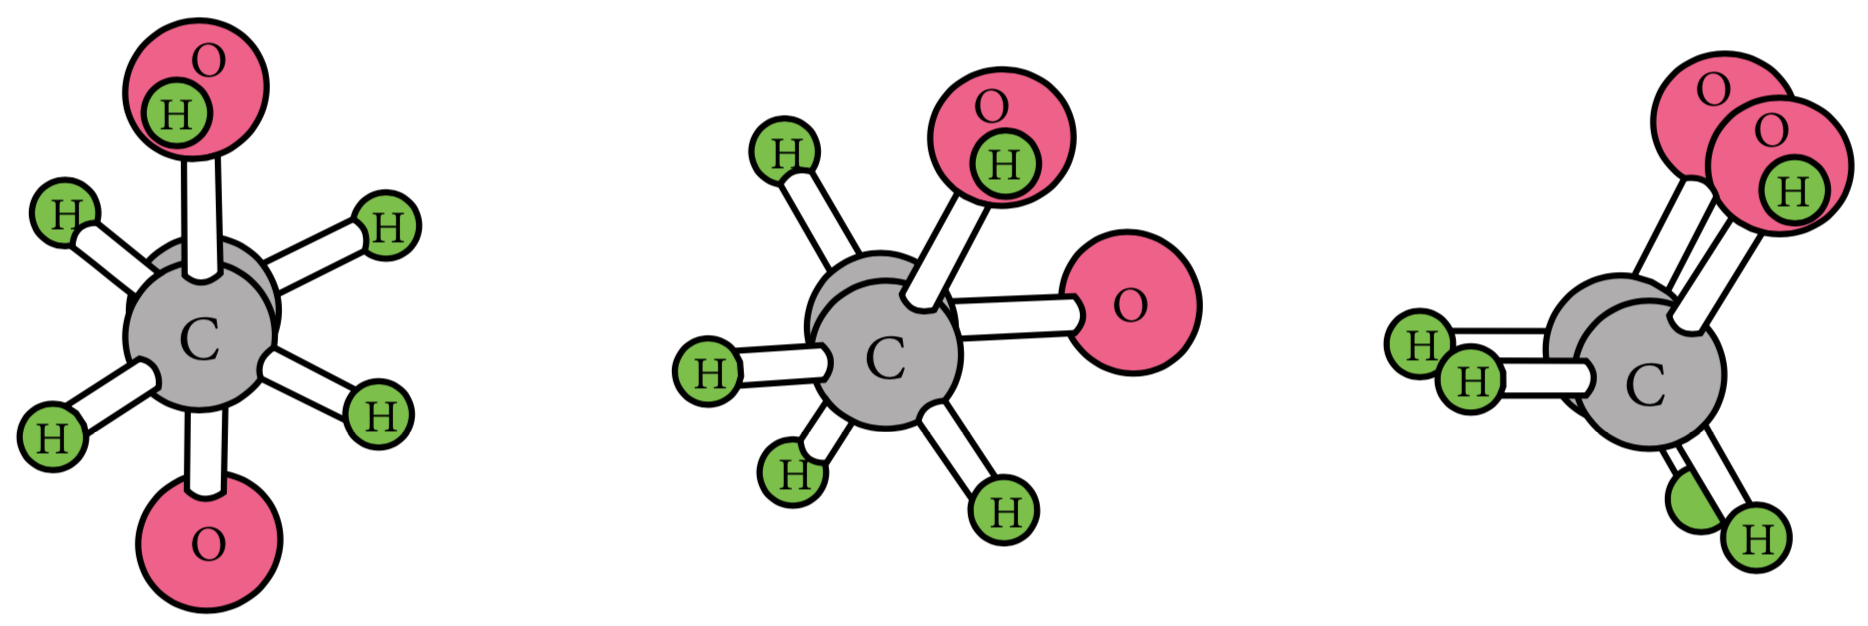
\includegraphics[width=0.9\textwidth]{coformers-1.png}

\caption{\small{Simple example of three coformers of ethylene glycol \cite{creighton2010biophysical}.}}

\label{fig:generation-of-microcan_state}
\end{minipage} 
\end{figure}

%Any conformation of a molecule of known covalent structure can be specified by the rotations about its single bonds, generally measured by either the torsion angle or the dihedral angle. In general, interactions between neighboring atoms, usually steric repulsions, mean that not all bond rotations have the same free energy and are equally probable
%\begin{figure}[h]
%\centering
%\begin{minipage}[t]{0.9\textwidth}
%\centering
%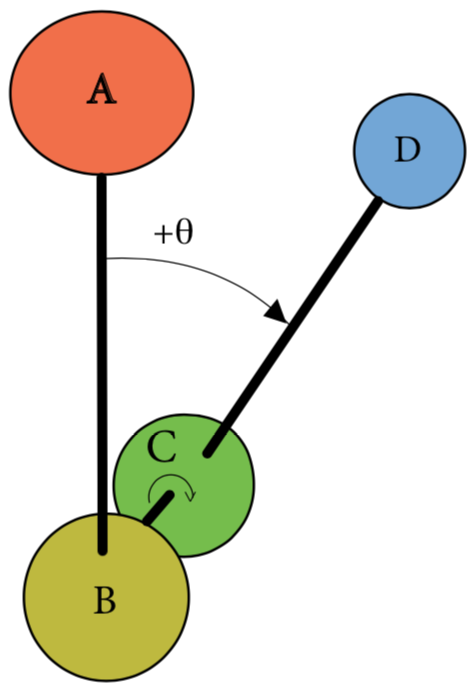
\includegraphics[width=0.22\textwidth]{./images/dihedral-0.png}
%\hspace{1cm}
%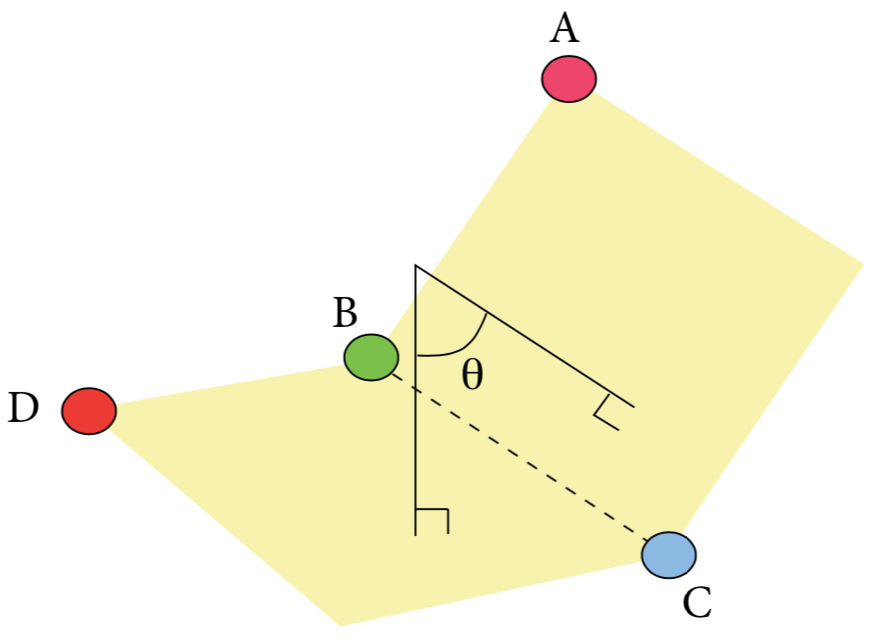
\includegraphics[width=0.45\textwidth]{./images/improper.png}
%
%\caption{\small{On the left: the torsion angles within a molecule that refer to the rotations about individual covalent bonds linking a pair of atoms; they are defined using two further atoms bonded to the first pair of atoms.  \cite{creighton2010biophysical}.}}
%
%\label{fig:generation-of-microcan_state}
%\end{minipage} 
%\end{figure}

A large biological macromolecule can have a stable, fixed 3-D structure, referred to as its native conformation, if it has sufficient stabilizing interactions between its various atoms. Although most of the conformation is fixed and it is considered a single conformation, parts of the molecule may still be flexible and able to undergo rotations about certain bonds. The average overall conformation can be considered a macro-conformation, whereas the variations resulting from flexibility define various micro-conformations. Interconverting different macro-conformations requires a cooperative change of a number of bond rotations simultaneously, whereas micro-conformations are interconverted by changes of just one or a few bond rotations. These cooperative changes will usually occur only slowly or infrequently under physiological conditions, although it can be speeded up dramatically under denaturing conditions. This relatively slow interconversion of the two macro-conformations is described as a conformational change, in which the macromolecule has been converted from one family of micro-conformations to an experimentally distinguishable family of other micro-conformations
\cite{creighton2010biophysical}.

In the case of a protein, its conformations will depend whether on the structures and conformational properties of their residues that on the environment -- especially the relative interactions of the protein with the solvent and with itself.

In this picture, the conformational entropy is a measure of the ability to adopt a number of such conformations that stabilizes the flexible state. A single conformation will be adopted only if the interactions stabilizing that particular conformation are sufficiently strong to overcome the conformational entropy tending to keep the protein unfolded. The number of micro-conformations and the conformational entropies of proteins can be very large. For example, if each residue can adopt an average of $j$ conformations, and there are $N$ residues in the protein, the total number of conformations possible will be approximately $j^N$. If the reasonable assumption is made that $j$ is $8$ and $N$ is $500$, there will be $8^{500}$ ($\approx 10^{452}$) conformations possible, a truly astronomical number. Of course, some of these conformations will not be feasible because they would have atoms of the protein overlapping in space, the excluded volume effect. There is still, however, much scope to be conservative and predict an astronomical number of conformations. For example, even a short protein of 100 residues in which each residue could adopt only two different conformations could adopt more than $10^{30}$ different protein conformations. If all these conformations have similar free energies, each would have only a very small probability of occurring in a molecule. At 25 %\textdegree 
$^\circ$ C, the free energy contribution of the conformational entropy for a protein in which each residue can adopt 10 conformations will be 1.36 $N$ kcal/mol. Consequently, for any one conformation to predominate will require, on average, stabilizing interactions $>$1.36 kcal/mol/residue. In the absence of such stabilizing interactions, a protein will tend to exist in many different conformations. However, proteins and nucleic acids are able to adopt single folded conformations that predominate. Such stable conformations can be considered macro-conformations, in contrast to the micro-conformations that are adopted only transiently \cite{creighton2010biophysical}.


In the last years, there is a growing interest in the protein configurational entropy as a major factor in controlling the protein activities associated with signaling, regulation, and recognition.

a field of a growing interest is the protein configurational entropy as a major factor in controlling the protein activities associated with signaling, regulation, and recognition.
In this context, \\
- copiare un po' dall'articolo koreano e da quello vecchio

\newpage

In this regard, it was a keen insight to suppose that the protein configurational entropy ($S_\text{config}$) may be characterized just by two terms, i.e., the conformational ($S_\text{conf}$) and vibrational ($S_\text{vib}$) components.
The conformational component is associated with the number of accessible free-energy wells, whereas the vibrational component reflects the average width of the individual wells. (Although they are often used interchangeably, we shall refer to ``conformational'' entropy as a subcategory of ``configurational'' entropy as just described.) -> questo perché nel processo di folding e unfolding $S_\text{vib} \simeq 0$ e quindi $S_\text{config} = S_\text{conf} + S_\text{vib} \simeq S_\text{conf}$

Dissecting $S_\text{config}$ into $S_\text{conf}$ and $S_\text{vib}$ enables one to characterize modulations of the free-energy landscape caused by intrinsic and extrinsic factors in simple terms; furthermore, it will facilitate the discovery of molecular mechanisms underlying protein activities (in particular, those of intrinsically disordered proteins).

Configurational entropy, however, is known as one of the most difficult thermodynamic quantities to estimate, and a significant amount of effort has been devoted to developing computational methods for dealing with this quantity. 

Here, we propose a computational approach from a different perspective that is based on the classification of protein
dynamics on the free-energy landscape into conformational and vibrational contributions (Figure 1). 


\cite{karplus1987configurational}

The aim of this thesis is to study 
\newpage

In this context, studying the association processes that bring to the formation of the binding between a protein and its ligand, it is possible to decompose the free energy of the association of the two molecules into a summation of favorable and unfavorable contributions. The mainly unfavorable contribution is due to the loss of the three translational and three rotational degrees of freedom that lead to a considerable decrease of the entropy of the system. Generally, it is assumed that this contribution is offset by favorable enthalpy of binding and entropic contributions, such as the hydrophobic effect, changes in the protonation state and solvent or counterion release. Nevertheless, there is another mechanism by which a significant amount of entropy can be recovered, namely, due to the creation of some new internal degrees of freedom in the complex \cite{tidor1994contribution}.

Indeed, because electrostatic interactions and hydrophobic bonds are not rigid or specific and the association is an outcome of such noncovalent interactions, the associating units (i.e. the protein and the ligand) have a considerable freedom of relative motion. This freedom, corresponding to an increase in flexibility for the complex and manifested by changes in its vibrational spectrum, is able to lead to a significant positive contribution for the entropy of the association (aside from the contribution from solvent effects, such as the hydrophobic effect) \cite{steinberg1963entropy}.

During the years, theoretical normal mode analyses, used to estimate this vibrational changes, have suggested that this effect is likely to be thermodynamically important and, in 2004, a first experimental determination of the vibrational changes has been achieved by Balog et al. Using inelastic neutron scattering, they showed that the vibrations of the complex soften significantly at low frequency (less then 2.5 meV) relative to the unbound protein. Deriving the resulting free-energy change from the variation in the density of states, they found that this effect contributes significantly to the binding equilibrium \cite{balog2004direct}.

Anyway, there remains much to learn about the various contributions to ligand binding free energies. Indeed, whether the vibrational softening effect seen here is general for protein-ligand interactions remains to be determined. The direct access to the vibrational density of states provided by inelastic neutron scattering holds promise for the study of vibrational thermodynamic changes in many biomolecular association processes \cite{balog2004direct}. 

Hence, to better understand this phenomena, in 2011 Balog et al., using computer simulations, recreated the system studied in the 2004 and reproduced the experimental results with an atomic detail normal-mode analysis to perform a characterization of the observed vibrational change.
With these simulations they obtain several interesting results concerning the nature of the vibrational changes in the specific protein-ligand complex studied\footnote{Some of these results concern the identification of the residues most affected by ligand binding and their contribution to protein compressibility \cite{balog2011vibrational}.}. However, as they report in their paper, these results cannot be generalized to other proteins and ligands since the effect depends on the strength of the interactions involved. 

Furthermore, the present analysis concentrates on the harmonic component of the dynamics.

oreover, they did not explain in detail the effect that the changes in the vibrational modes of the complex have in the vibrational spectrum of the hydration water.


%\section{Experimental evidence - A brief overview of the neutron scattering results}
